\section{Results and Discussion} \label{sec:results}

\subsection{Tree Reconstruction Quality}

\begin{figure}
  \centering
  \begin{subfigure}[b]{\linewidth}
    \centering
    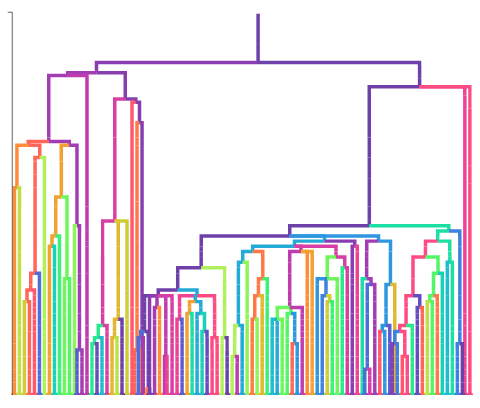
\includegraphics[width=\textwidth, height=0.13\textheight]{img/reference}
    \caption{%
      reference tree}
    \label{fig:plain-perfect-and-reconstruction-phylogenies:reference}
  \end{subfigure}
  \begin{subfigure}[b]{\linewidth}
    \centering
    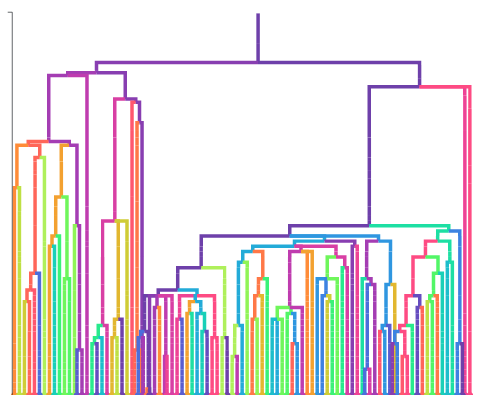
\includegraphics[width=\textwidth, height=0.13\textheight]{img/plain_resolution_100}
    \caption{%
      1\% resolution}
    \label{fig:plain-perfect-and-reconstruction-phylogenies:resolution_100}
  \end{subfigure}
  \begin{subfigure}[b]{\linewidth}
    \centering
    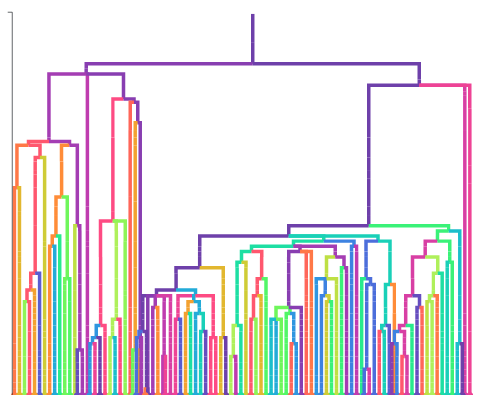
\includegraphics[width=\textwidth, height=0.13\textheight]{img/plain_resolution_30}
    \caption{%
      3\% resolution}
    \label{fig:plain-perfect-and-reconstruction-phylogenies:resolution_30}
  \end{subfigure}
  \begin{subfigure}[b]{\linewidth}
    \centering
    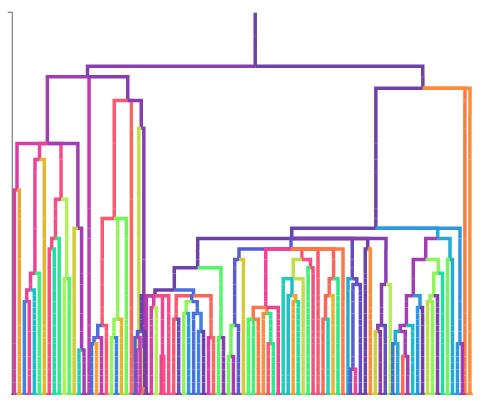
\includegraphics[width=\textwidth, height=0.13\textheight]{img/plain_resolution_10}
    \caption{%
      10\% resolution}
    \label{fig:plain-perfect-and-reconstruction-phylogenies:resolution_10}
  \end{subfigure}
  % \begin{noindent}
  \begin{subfigure}[b]{\linewidth}
    \centering
    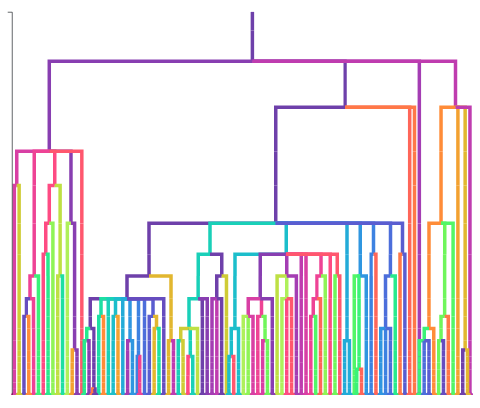
\includegraphics[width=\textwidth, height=0.13\textheight]{img/plain_resolution_3} \caption{%
      33\% resolution}
    \label{fig:plain-perfect-and-reconstruction-phylogenies:resolution_3}
  \end{subfigure}
  % \end{noindent}
  \caption{%
  \textbf{Comparison of phylogeny reconstructions across different hereditary stratigraphy resolutions in the plain evolutionary regime.}
    To maintain visual legibility, these trees contain the same sub-sample of 100 leaf nodes out of the 32,768 in the full trees.
    Sub-figures are arranged from top to bottom in coarsening order of reconstruction resolution.
    Taxon and branch color coding is consistent across subpanels.
    Visit \url{mmore500.com/hstrat-evolutionary-inference/} for mouseover-based highlighting of corresponding clades between reconstructions and reference.
  }
  \label{fig:plain-perfect-and-reconstruction-phylogenies}
\end{figure}


mean/std/max
plain	1% resolution	epoch=7+mut_distn=np.random.standard_normal	-2.10425894221959E-14	1.50722607904943E-16	-2.08295182385988E-14
plain	10% resolution	epoch=7+mut_distn=np.random.standard_normal	-2.10469692847644E-14	1.55963069867711E-16	-2.08314605325639E-14
plain	3% resolution	epoch=7+mut_distn=np.random.standard_normal	-2.10620443554657E-14	1.51986960038139E-16	-2.08462322970661E-14
plain	33% resolution	epoch=7+mut_distn=np.random.standard_normal	-2.10637937229546E-14	1.4397013470276E-16	-2.08299428020224E-14


spatial structure	1% resolution	epoch=7+mut_distn=np.random.standard_normal	7.81849234344143E-07	4.14508890707294E-06	2.82106734844714E-05
spatial structure	10% resolution	epoch=7+mut_distn=np.random.standard_normal	0.00275016417111772	0.0106125775395443	0.0533132541036293
spatial structure	3% resolution	epoch=7+mut_distn=np.random.standard_normal	0.000857215705953448	0.00540569979603497	0.0380983817532154
spatial structure	33% resolution	epoch=7+mut_distn=np.random.standard_normal	0.00763527603510759	0.0149106058655545	0.0584668625701303

mean, std, and max quartet error summary statistics for each reconstruction regime/resolution are provided in Supplementary Table TODO


KRUSKAL WALLIS by resolution
% 38 	50 	4 	quartet_distance 	17.612788 	5.285933e-04 	spatial structure 	7 	np.random.standard_normal
%
% 31 	50 	4 	quartet_distance 	11.319749 	1.011675e-02 	spatial structure 	7 	np.random.exponential
%
% 23 	50 	4 	quartet_distance 	9.640107 	2.188663e-02 	plain 	2 	np.random.standard_normal
% 24 	50 	4 	quartet_distance 	148.020119 	7.044412e-32 	spatial structure 	2
% np.random.standard_normal
%
% 50 	4 	quartet_distance 	100.829421 	1.030737e-21 	weak selection 	0 	np.random.standard_normal

Full statistical results are in Supplementary Table TODO

KRUSKAL WALLIS by regime for each resolution

SIGNIFICANT $p < 0.02$ over all regimes for all resolutions and all sensitivity analysis variables


\subsection{Phylometrics by Evolutionary Regime}

figure: boxplot
\begin{teaserfigure}
  \centering
  % \begin{noindent}
  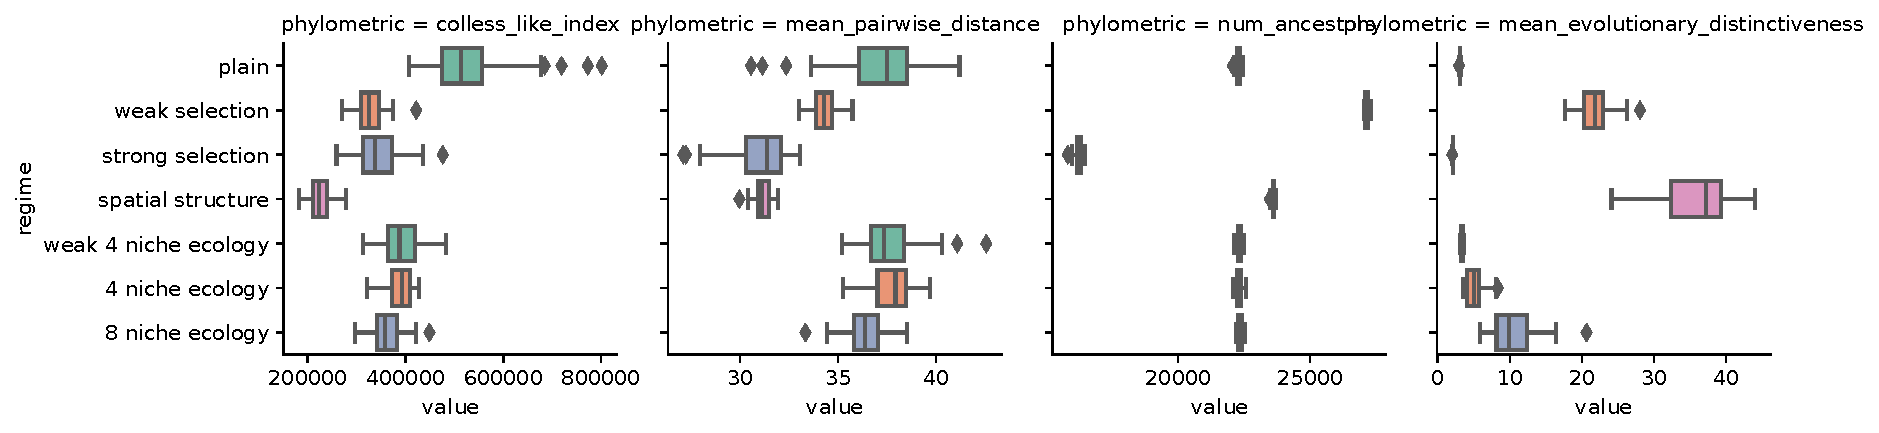
\includegraphics[width=\textwidth]{binder/binder/teeplots/col=phylometric+epoch=7+mut_distn=np.random.standard_normal+viz=boxplot+x=value+y=regime+ext=.pdf}
  % \end{noindent}
  \caption{%
    Distribution of phylometrics measured with perfect phylogenetic tracking across surveyed evolutionary regimes ($n=50$).
  }
  \label{fig:perfect-tree-phylometrics}
\end{teaserfigure}


Supplementary Figure \ref{fig:perfect-tree-phylometrics-sensitivity-analysis}

\begin{teaserfigure}
  \centering
  % \begin{noindent}
  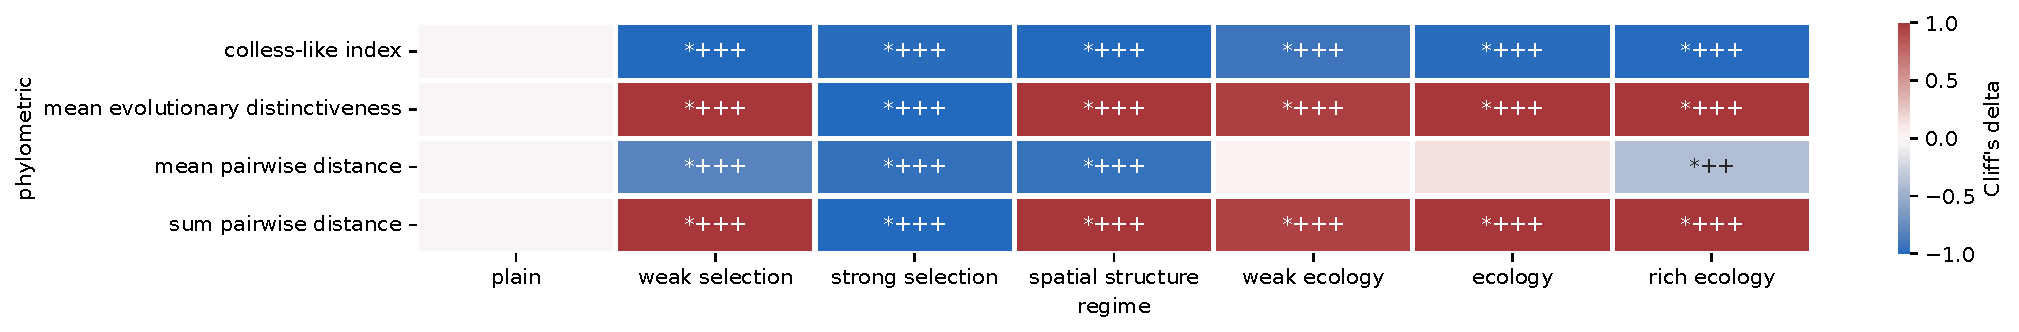
\includegraphics[width=\textwidth]{binder/binder/teeplots/epoch=7+mut_distn=np.random.standard_normal+viz=heatmap+x=regime+y=phylometric+ext=.pdf}
  % \end{noindent}
  \caption{%
    Phylogenetic metric values across surveyed evolutionary conditions, relative to plain regime.
  }
  \label{fig:perfect-tree-phylometrics}
\end{teaserfigure}


statistics
We first tested whether each phylometric showed significant variance among the seven tested regimes. For all variables across all sensitivity analysis conditions, we found very strong evidence that this was the case (Kruskal-Wallis tests; all $p < 1\times10^{-50}$; $n=50$ per condition for all 7 conditions; Supplementary Table TODO).

Next, we performed an all-pairs comparison between the seven surveyed evolutionary regimes for all phylometrics (Wilcoxon test with Bonferoni correction; corrected significance threshold $1.49 \times 10^{-4}$; $n=50$ per condition; 84 comparisons per sensitivity analysis condition; 336 comparisons total). We found significant differences for all metrics except

results at epoch 7
    \begin{itemize}
        \item plain	4 niche ecology	50	mean pairwise distance
        \item plain	4 niche ecology	50	num ancestors
        \item plain	8 niche ecology	50
        \item mean pairwise distance
        \item plain	8 niche ecology	50	num ancestors
        \item strong selection	8 niche ecology	50
        \item colless like index
        \item strong selection	spatial structure	50	mean pairwise distance
        \item weak 4 niche ecology	4 niche ecology	50	colless like index
        \item weak 4 niche ecology	4 niche ecology	50	mean pairwise distance
        \item weak 4 niche ecology	4 niche ecology	50	num ancestors
        \item weak 4 niche ecology	8 niche ecology	50	num ancestors
        \item weak 4 niche ecology	plain	50	mean pairwise distance
        \item weak 4 niche ecology	plain	50	num ancestors
        \item weak selection	strong selection	50	colless like index
    \end{itemize}

results at epoch 0
\begin{itemize}
\item 4 niche ecology	weak 4 niche ecology	50	colless like index
\item 4 niche ecology	weak 4 niche ecology	50	mean pairwise distance
\item 4 niche ecology	weak 4 niche ecology	50	num ancestors
\item 8 niche ecology	4 niche ecology	50	num ancestors
\item 8 niche ecology	weak 4 niche ecology	50	num ancestors
\item plain	4 niche ecology	50	mean pairwise distance
\item plain	4 niche ecology	50	num ancestors
\item plain	8 niche ecology	50
\item mean pairwise distance
\item plain	8 niche ecology	50	num ancestors
\item plain	weak 4 niche ecology	50	mean pairwise distance
\item plain	weak 4 niche ecology	50	num ancestors
\item spatial structure	weak selection	50	mean evolutionary distinctiveness
\item strong selection	4 niche ecology	50	colless like index
\item strong selection	8 niche ecology	50	colless like index

\end{itemize}

results at epoch 2
\begin{itemize}
    \item 8 niche ecology	4 niche ecology	50	num ancestors
    \item 8 niche ecology	weak 4 niche ecology	50	num ancestors
    \item plain	4 niche ecology	50	mean pairwise distance
    \item plain	4 niche ecology	50	num ancestors
    \item plain	8 niche ecology	50	mean pairwise distance
    \item plain	weak 4 niche ecology	50	mean pairwise distance
    \item plain	weak 4 niche ecology	50	num ancestors
    \item strong selection	8 niche ecology	50	colless like index
\item strong selection	spatial structure	50	mean pairwise distance
\item weak 4 niche ecology	4 niche ecology	50	colless like index
\item weak 4 niche ecology	4 niche ecology	50	mean pairwise distance
\item weak 4 niche ecology	4 niche ecology	50	num ancestors
\item weak selection	strong selection	50	colless like index

\end{itemize}

results at epoch 7, exponential
    \begin{itemize}
        \item 4 niche ecology	8 niche ecology	50	colless like index
        \item 4 niche ecology	8 niche ecology	50	num ancestors
        \item 4 niche ecology	weak 4 niche ecology	50	colless like index
        \item 4 niche ecology	weak 4 niche ecology	50	mean pairwise distance
        \item 4 niche ecology	weak 4 niche ecology	50	num ancestors
        \item plain	4 niche ecology	50	mean pairwise distance
        \item plain	4 niche ecology	50	num ancestors
        \item plain	8 niche ecology	50	mean pairwise distance
        \item plain	weak 4 niche ecology	50	mean pairwise distance
        \item plain	weak 4 niche ecology	50	num ancestors
        \item weak 4 niche ecology	8 niche ecology	50	num ancestors
        \item weak selection	4 niche ecology	50	colless like index
        \item weak selection	8 niche ecology	50	colless like index
        \item weak selection	8 niche ecology	50	mean pairwise distance
        \item weak selection	plain	50	mean pairwise distance
        \item 4 niche ecology	8 niche ecology	50	num ancestors

    \end{itemize}
\subsection{Phylometrics with Spatial Structure Nuisance}

We first tested whether each phylometric showed significant variance among the four tested regimes. For all variables across all sensitivity analysis conditions, we found very strong evidence that this was the case (Kruskal-Wallis tests; all $p < 1\times10^{-20}$; $n=50$ per condition for all 4 conditions; Supplementary Table TODO).

Next, we performed an all-pairs comparison between the seven surveyed evolutionary regimes for all phylometrics (Wilcoxon test with Bonferoni correction; corrected significance threshold $5.26 \times 10^{-4}$; $n=50$ per condition; 24 comparisons per sensitivity analysis condition; 96 comparisons total). We found significant differences for all metrics except

epoch 7
\begin{itemize}
    \item 4 niche ecology	plain	49	colless like index
\item weak 4 niche ecology	4 niche ecology	49	num ancestors
\end{itemize}

epoch 0
\begin{itemize}

\item plain	weak 4 niche ecology	50	colless like index
\item plain	weak 4 niche ecology	50	mean pairwise distance
\item weak 4 niche ecology	4 niche ecology	50	num ancestors

\end{itemize}

epoch 2
\begin{itemize}
    \item weak 4 niche ecology	4 niche ecology	50	num ancestors
\end{itemize}

exponential
\begin{itemize}
    \item 4 niche ecology	plain	50	colless like index
    \item 4 niche ecology	plain	50	mean pairwise distance
    \item 4 niche ecology	weak 4 niche ecology	50	num ancestors
\end{itemize}

figure boxplot
\begin{figure*}
  \centering
  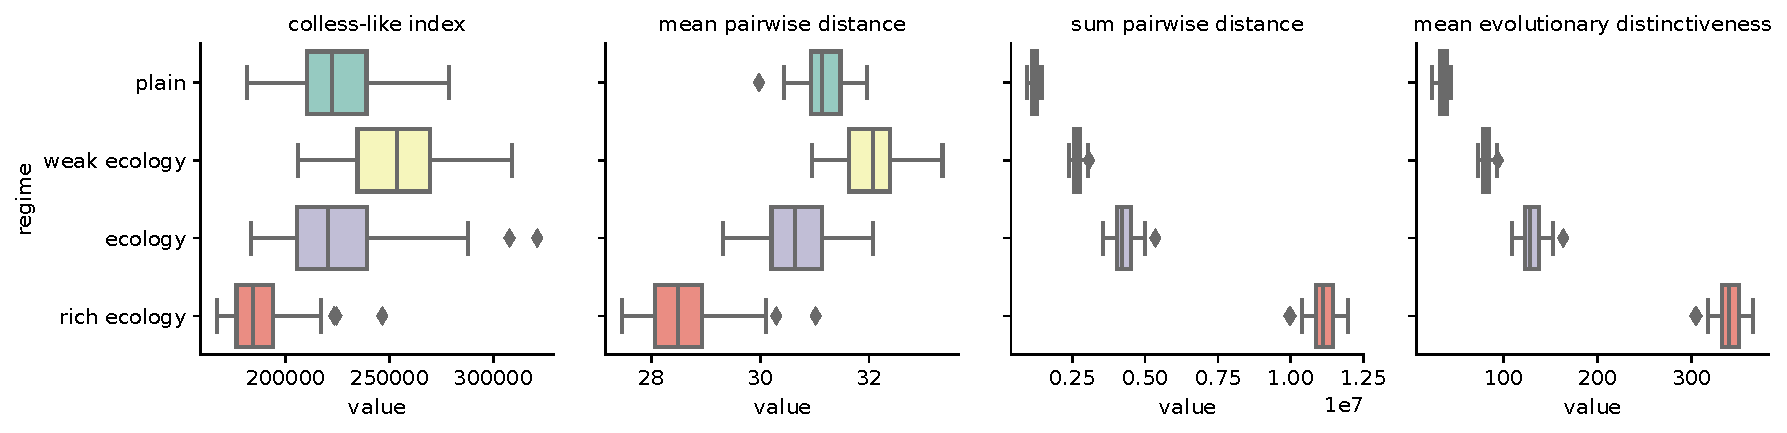
\includegraphics[width=\textwidth]{binder/binder/teeplots/col=phylometric+epoch=7+mut_distn=np.random.standard_normal+nuisance=spatial-structure+viz=boxplot+x=value+y=regime+ext=.pdf}
  \caption{TODO}
  \label{fig:perfect-tree-phylometrics-with-spatial-nuisance}
\end{figure*}


\subsection{Phylometrics with Reconstruction Error Nuisance}

\begin{sidewaysfigure*}
  \centering
  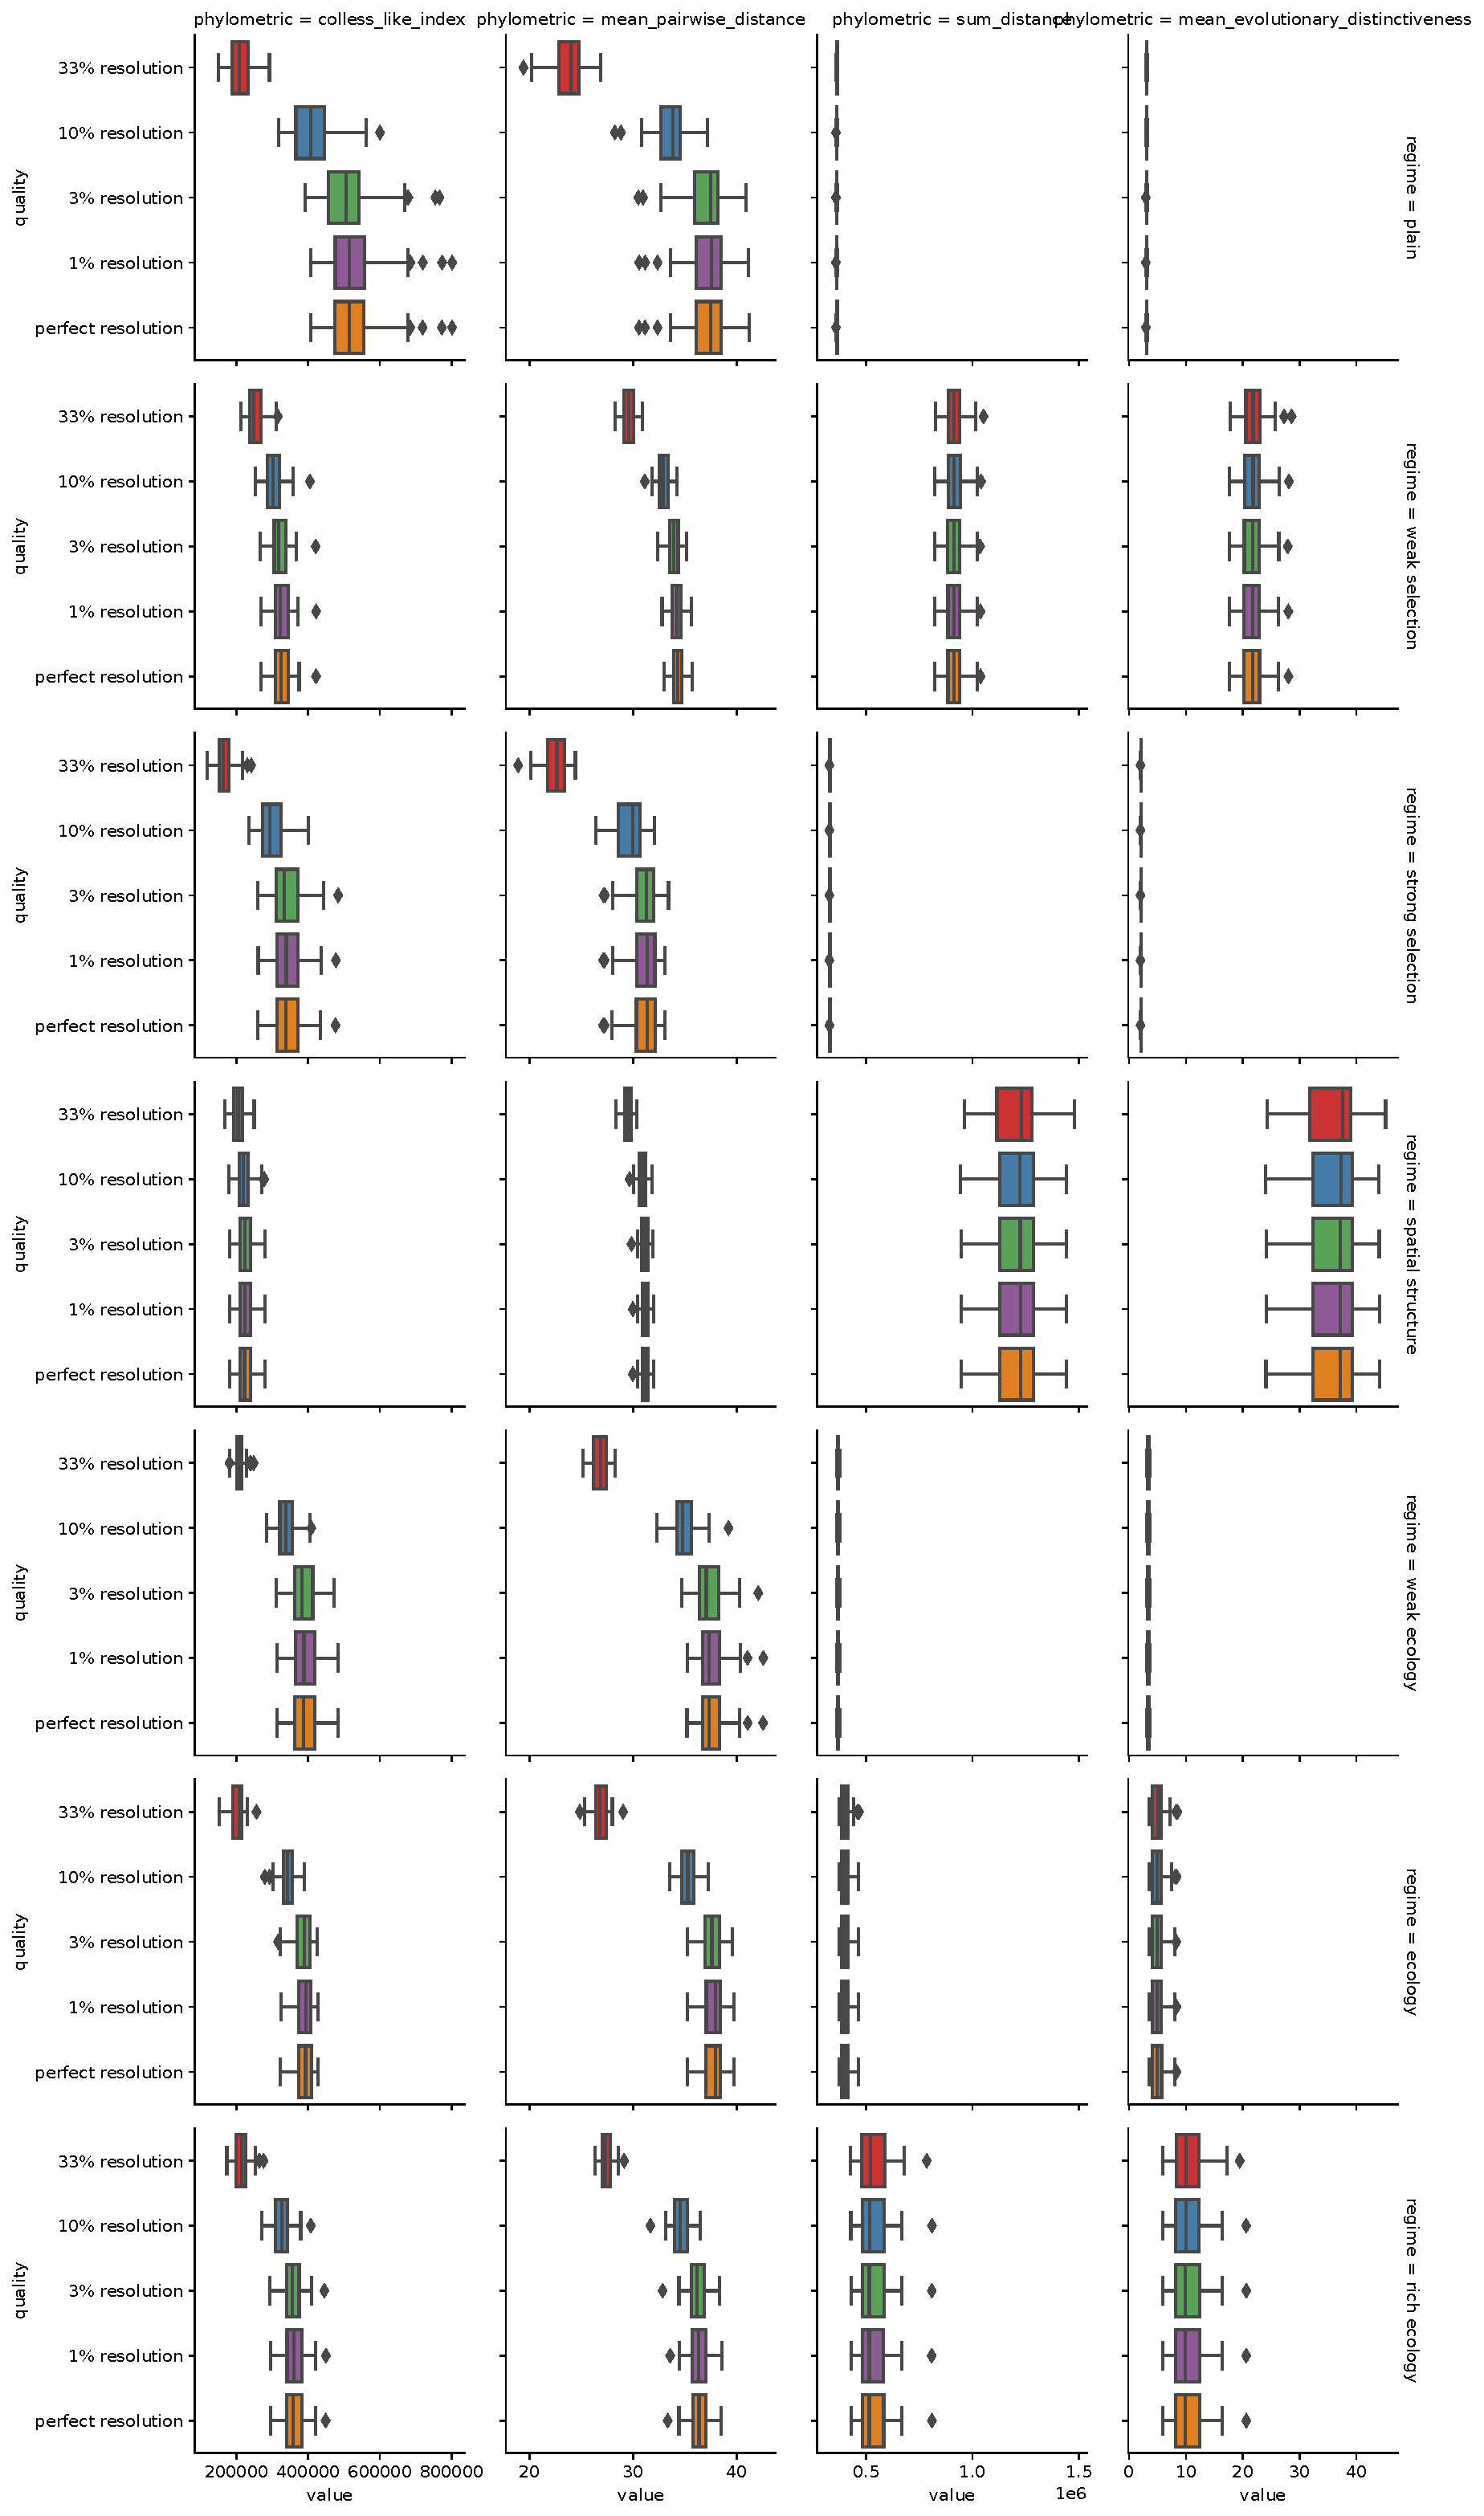
\includegraphics[height=\textwidth,angle=-90,origin=c]{binder/binder/teeplots/col=phylometric+epoch=7+mut_distn=np.random.standard_normal+row=regime+viz=boxplot+x=value+y=quality+ext=.pdf}
  \caption{TODO}
  \label{fig:reconstructed-tree-phylometrics}
\end{sidewaysfigure*}


figure facet boxplot

STATISTICS: do phylometrics vary by resolution for each regime?
TODO

\begin{figure*}
  \centering
  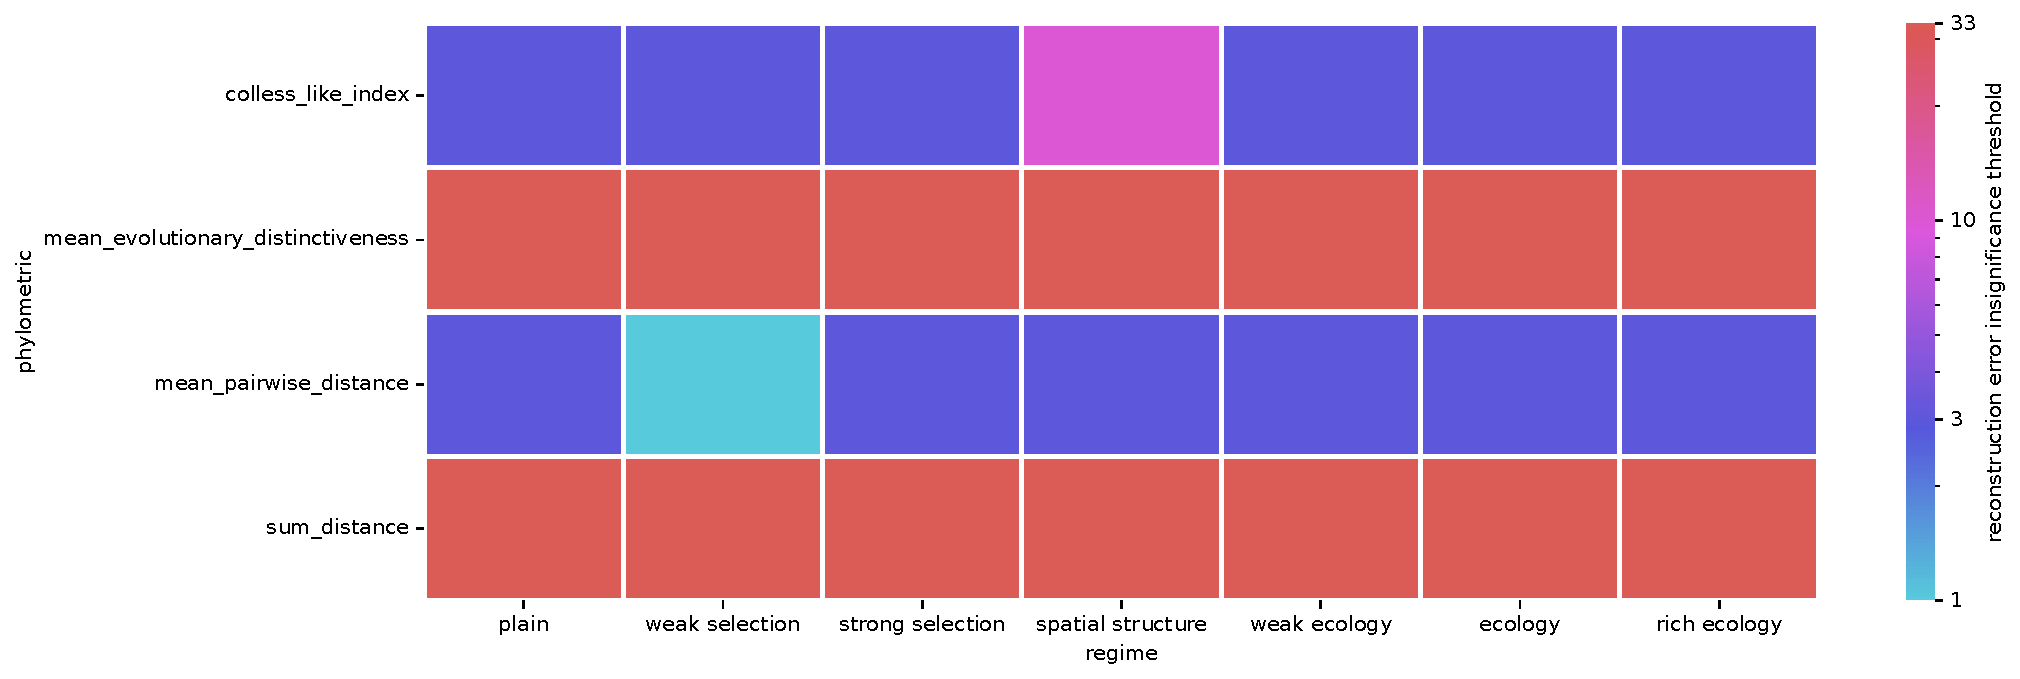
\includegraphics[width=\textwidth]{binder/binder/teeplots/epoch=7+hue=quality-threshold+mut_distn=np.random.standard_normal+viz=heatmap+x=regime+y=phylometric+ext=.pdf}
  \caption{TODO}
  \label{fig:reconstructed-tree-phylometrics-error}
\end{figure*}


Supplementary Figure \ref{fig:reconstructed-tree-phylometrics-error-sensitivity-analysis}.

\subsection{Phylometrics with Spatial Structure and Reconstruction Error Nuisances}

figure facet boxplot
\begin{figure*}
  \centering
  % \begin{noindent}
  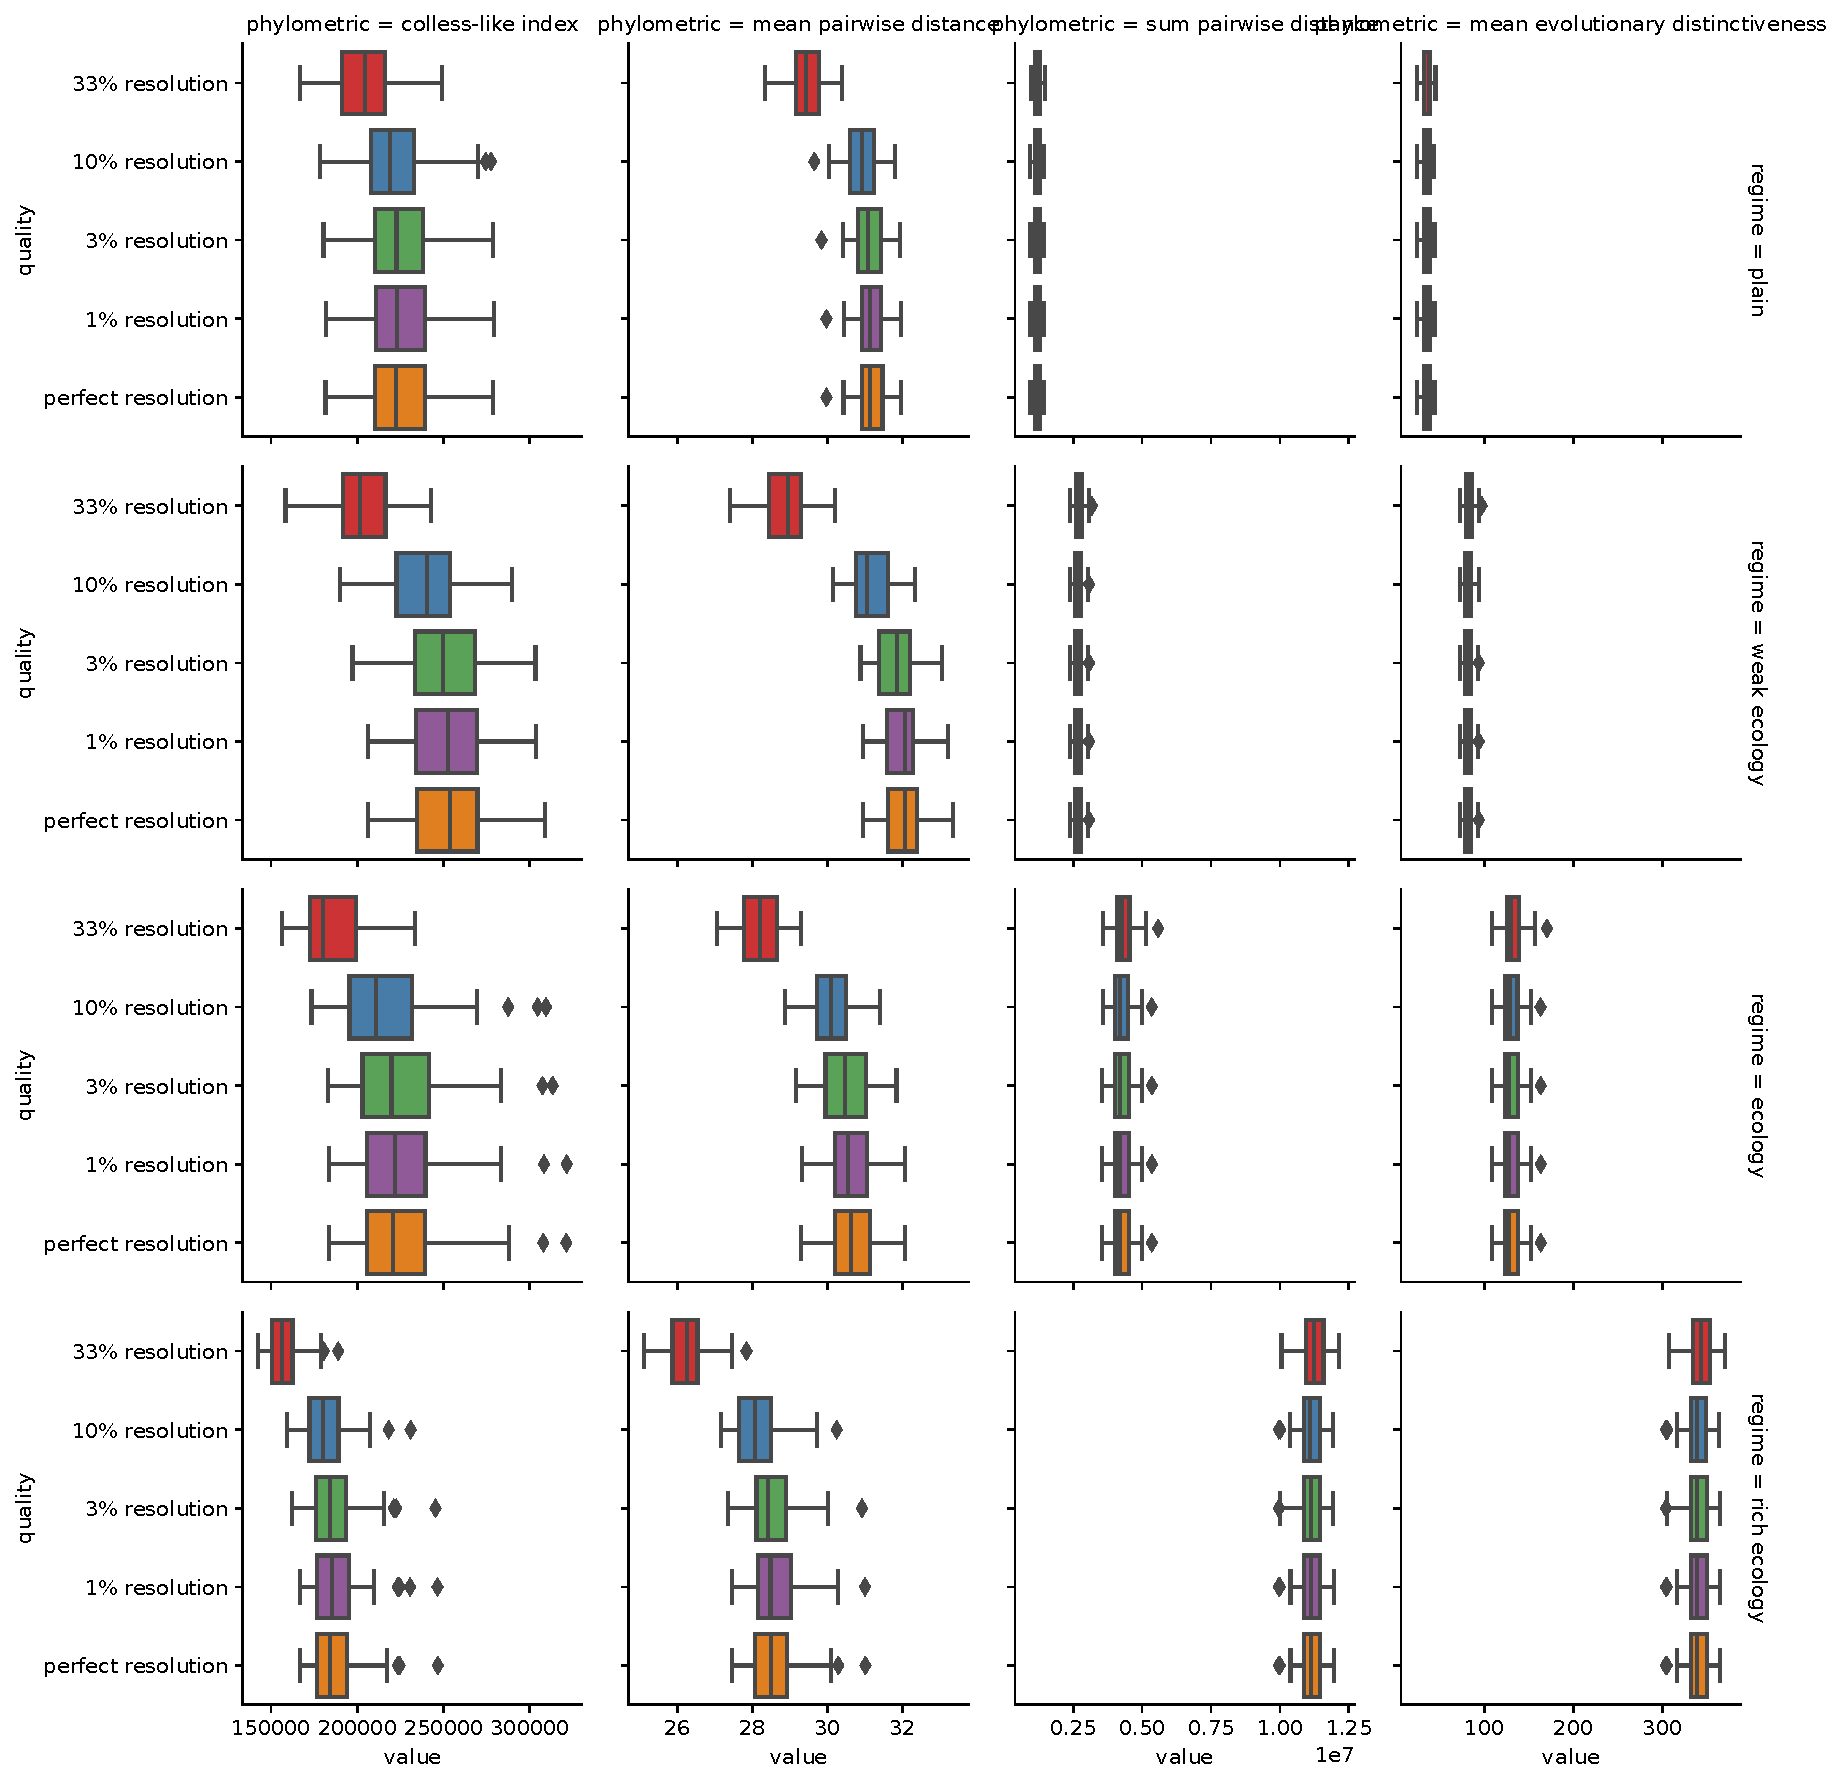
\includegraphics[width=\textwidth]{binder/binder/teeplots/col=phylometric+epoch=7+mut_distn=np.random.standard_normal+nuisance=spatial-structure+row=regime+viz=boxplot+x=value+y=quality+ext=.pdf}
  % \end{noindent}
  \caption{%
    Distributions of phylometrics across surveyed reconstruction fidelities for evolutionary regimes with underlying spatial structure (i.e., 1,024 niches).
    Results are for standard experimental conditions: gaussian mutation distribution at epoch 7 (generation 262,144).
    See Figures \labelcref{fig:reconstructed-tree-phylometrics-with-spatial-nuisance-epoch0,fig:reconstructed-tree-phylometrics-with-spatial-nuisance-epoch2,fig:reconstructed-tree-phylometrics-with-spatial-nuisance-exponential} for results under sensitivity analysis conditions.
    Sample sizes of $n=50$ replicates define each depicted distribution.
  }
  \label{fig:reconstructed-tree-phylometrics-with-spatial-nuisance}
\end{figure*}


STATISTICS: do phylometrics vary by resolution for each regime?
TODO